\subsection{Student Grades}

\subsubsection{Statement}
Write a program in C that uses a two-dimensional array to store the numeric grade for
each student (n) in a multiple teacher’s class (m). The program assumes that the teacher has three
classes and a maximum of 30 students per class. Both the variable M and N should be user
defined.

\subsubsection{Code}
\begin{minted}{c} 
 
#include <stdio.h>

struct student
{
  char grade;
};

void get_marks(student classes[][30])
{
  int m, n;

  printf("\nEnter class: ");
  scanf("%d", &m);
  printf("Enter student: ");
  scanf("%d", &n);

  printf("The given student has got %c grade!\n", classes[m - 1][n - 1]);
}

void populate_classes(student classes[3][30])
{
  int num;

  for (int i = 0; i < 3; i++)
  {
    student *curr_class = classes[i];
    printf("Enter number of students in class %d: ", i + 1);
    scanf("%d", &num);

    for (int j = 0; j < num; j++)
    {
      printf("Enter the Grade of student %d in class %d: ", j + 1, i + 1);
      scanf(" %c", &(curr_class[j].grade)); // blank space is important
    }
    printf("\n");
  }
}

int main(int argc, char const *argv[])
{

  student classes[3][30];

  populate_classes(classes);
  get_marks(classes);

  return 0;
}

\end{minted}

\subsubsection{Output}
\begin{figure}[!htb]
  \centering
  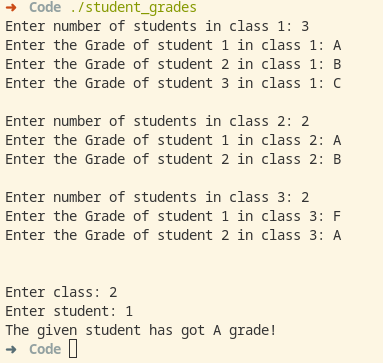
\includegraphics[width=4in]{Images/1.png}
  \label{output:1}
  \caption{Output: 1}
\end{figure}

\pagebreak
\subsection{Average Age}

\subsubsection{Statement}
Write the program to input the value of age of employees in the company. You have to
calculate the average age of the employee in the company using pointer of array.

\subsubsection{Code}
\begin{minted}{c} 

#include <stdio.h>
#include <stdlib.h>

float avg(int arr[], int n)
{
  float sum = 0;
  for (int i = 0; i < n; i++)
    sum += arr[i];
  return sum / (float)n;
}

int main(int argc, char const *argv[])
{
  int n;
  printf("Enter number of employees: ");
  scanf("%d", &n);

  int *employees = (int *)malloc(n * sizeof(int));

  for (int i = 0; i < n; i++)
  {
    printf("Enter age of employee %d: ", i + 1);
    scanf("%d", &employees[i]);
  }

  printf("The average age of employees is = %.2f\n", avg(employees, n));

  free(employees);

  return 0;
}

\end{minted}

\pagebreak
\subsubsection{Output}
\begin{figure}[!htb]
  \centering
  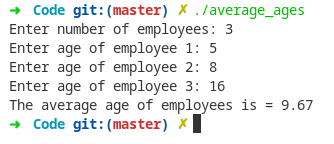
\includegraphics[width=4in]{Images/average.png}
  \label{output:2}
  \caption{Output: 2}
\end{figure}


\pagebreak
\subsection{Length of string}

\subsubsection{Statement}
A user has given a random size string to input, you have to calculate the length of the
string using pointer. You cannot use predefined function strrev.

\subsubsection{Code}
\begin{minted}{c} 
#include <stdio.h>
int main()
{
  char str[100], i;
  printf("Enter a string: ");
  scanf("%[^\n]s", str);

  // '\0' represents end of String
  for (i = 0; str[i] != '\0'; ++i);
  printf("\nLength of input string: %d\n", i);

  return 0;
}
\end{minted}
\subsubsection{Output}
\begin{figure}[!htb]
  \centering
  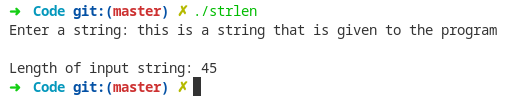
\includegraphics[width=4in]{Images/strlen.png}
  \label{output:3}
  \caption{Output: 3}
\end{figure}

\pagebreak
\subsection{Start-Up Owner}

\subsubsection{Statement}
A start-up owner is interested to maintain the dataset of the newly recruited employees.

She is interested in storing the Emp\_Name (Str), Emp\_Age (int), Emp\_Degree (Str), Emp\_Exp
(Float), Emp\_add (Structure). Emp\_add needs one user defined data to store street no, city,
district and state for the employee address. You have to design a database where we can store all
the information for at least 20 employees.

\subsubsection{Code}
\begin{minted}{c} 
#include <stdio.h>

struct address
{
  int street;
  char city[50];
  char district[50];
  char state[50];
};

struct employee
{
  char Emp_Name[50];
  int Emp_Age;
  char Emp_Degree[50];
  float Emp_Exp;
  address Emp_add;
};

void add_emploee(employee &Employee, int i)
{
  printf("\nEnter Name of employee %d: ", i);
  scanf("%s", &Employee.Emp_Name);
  printf("Enter Age of employee %d: ", i);
  scanf("%d", &Employee.Emp_Age);
  printf("Enter Degree of employee %d: ", i);
  scanf("%s", &Employee.Emp_Degree);
  printf("Enter Experience of employee %d: ", i);
  scanf("%f", &Employee.Emp_Exp);

  printf("*Address Details*\n");
  printf("Enter City of employee %d: ", i);
  scanf("%s", &Employee.Emp_add.city);
  printf("Enter District of employee %d: ", i);
  scanf("%s", &Employee.Emp_add.district);
  printf("Enter State of employee %d: ", i);
  scanf("%s", &Employee.Emp_add.state);
  printf("Enter Street of employee %d: ", i);
  scanf("%d", &Employee.Emp_add.street);
}

void print_employee(employee Employee)
{
  printf("\n%s %s %s", Employee.Emp_Name, Employee.Emp_Degree, Employee.Emp_add.city);
}

int main(int argc, char const *argv[])
{
  int n;
  printf("Enter Number of employees: ");
  scanf("%d", &n);

  employee Employees[n];

  for (int i = 0; i < n; i++)
    add_emploee(Employees[i], i + 1);

  for (int i = 0; i < n; i++)
    print_employee(Employees[i]);
  return 0;
}

\end{minted}
\pagebreak
\subsubsection{Output}
\begin{figure}[!htb]
  \centering
  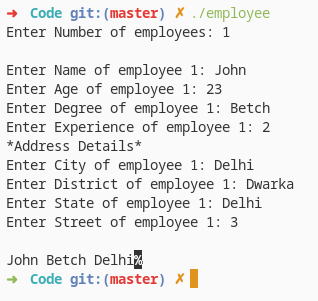
\includegraphics[width=4in]{Images/employee.png}
  \label{output:4}
  \caption{Output: 4}
\end{figure}


\pagebreak
\subsection{Student Names}

\subsubsection{Statement}
Defined a two-dimensional matrix (char)[50][20] to store the student’s name in the class.
We are expecting to store the 50 students with different length name. Write a program to print all
the name with the help of pointers

\subsubsection{Code}
\begin{minted}{c} 
#include <stdio.h>

void print_names(char students[][20], int n)
{
  printf("\nStudents are: \n");
  for (int i = 0; i < n; i++)
    printf("%s\n", students[i]);
}

int main(int argc, char const *argv[])
{
  int n;
  char students[50][20];
  printf("Enter a number: ");
  scanf("%d", &n);

  for (int i = 0; i < n; i++)
  {
    printf("Enter the name for student %d: ", i + 1);
    scanf("%s", students[i]);
  }
  print_names(students, n);
  return 0;
}

\end{minted}
\subsubsection{Output}
\begin{figure}[!htb]
  \centering
  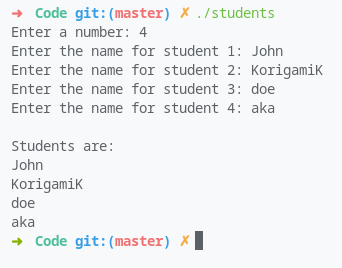
\includegraphics[width=4in]{Images/student_names.png}
  \label{output:5}
  \caption{Output: 5}
\end{figure}

\pagebreak
\subsection{XOR Operation}

\subsubsection{Statement}
The outcome of a XOR operation is true if and only if one operand (but not both) is true. Write
a program in 'C' which returns the outcome of an Exclusive OR operation performed on its two
operands

\subsubsection{Code}
\begin{minted}{c} 
#include <stdio.h>

int main(int argc, char const *argv[])
{
  int a, b;
  printf("Enter 2 numbers:\n");
  scanf("%d", &a);
  scanf("%d", &b);
  int xor_result = (a | b) & (~(a & b));
  printf("The XOR of %d and %d is equal to %d\n", a, b, xor_result);
  return 0;
}

\end{minted}
\subsubsection{Output}
\begin{figure}[!htb]
  \centering
  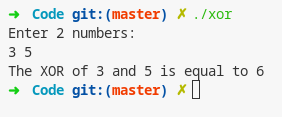
\includegraphics[width=4in]{Images/xor.png}
  \label{output:6}
  \caption{Output: 6}
\end{figure}


\pagebreak
\subsection{Left and Right Shift}

\subsubsection{Statement}
Write a program in C to show that Right shift effectively divides a number by 2 and a left shift
effectively multiplies a number by 2

\subsubsection{Code}
\begin{minted}{c} 
#include <stdio.h>

int main(int argc, char const *argv[])
{
  int a;
  printf("Enter a numbers: ");
  scanf("%d", &a);

  for (int i = 0; i < 4; i++)
    printf("%d Right shifted %d times is equal to %d\n", a, i, a >> i);
  printf("\n");
  for (int i = 0; i < 4; i++)
    printf("%d Left shifted %d times is equal to %d\n", a, i, a << i);

  return 0;
}

\end{minted}
\subsubsection{Output}
\begin{figure}[!htb]
  \centering
  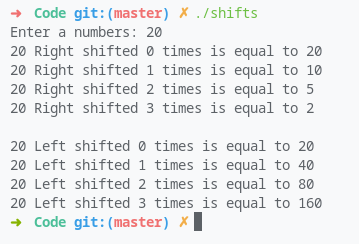
\includegraphics[width=4in]{Images/shifts.png}
  \label{output:7}
  \caption{Output: 7}
\end{figure}


\pagebreak
\subsection{Magic Number}

\subsubsection{Statement}
Using the ? Operator, rewrite the magic number program discussed in the class

\subsubsection{Code}

\subsubsection{Output}

\pagebreak
\subsection{Quotient}
\subsubsection{Statement}
Using if else statement write a program in ‘C’ to read two integers from the user and display
the quotient. Your program should be able to detect divide by zero.
\subsubsection{Code}
\begin{minted}{c} 
#include <stdio.h>

int main(int argc, char const *argv[])
{
  float a, b;
  printf("Enter 2 numbers:\n");
  scanf("%f", &a);
  scanf("%f", &b);
  b == 0 
    ? printf("Undefined Behavior\n") 
    : printf("The quotient is: %.2f\n", a / b);
  return 0;
}

\end{minted}
\subsubsection{Output}
\begin{figure}[!htb]
  \centering
  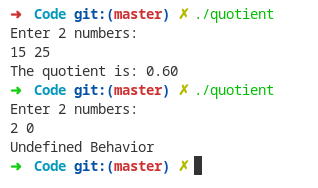
\includegraphics[width=4in]{Images/quotient.png}
  \label{output:9}
  \caption{Output: 9}
\end{figure}


\pagebreak
\subsection{Text File}
\subsubsection{Statement}
Write a program in C that inputs lines of text until a blank line is entered. Then it redisplays
each line one character at a time
\subsubsection{Code}
\begin{minted}{c} 
#include <stdio.h>
int main(int argc, char const *argv[])
{
  char x, text[100];
  int i = 0;
  while (x = getchar())
  {
    if (x == '\n')
    {
      for (int j = 0; j < i; j++)
        printf("%c\n", text[j]);
      break;
    }
    else
      text[i] = x;
    i++;
  }

  return 0;
}

\end{minted}
\subsubsection{Output}
\begin{figure}[!htb]
  \centering
  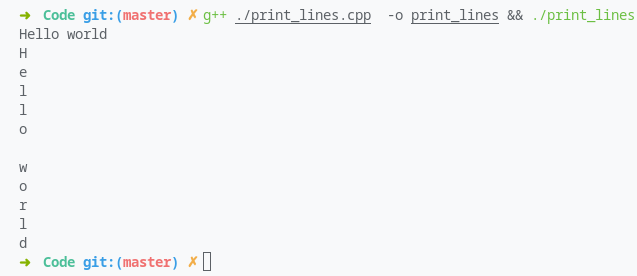
\includegraphics[width=4in]{Images/print_lines.png}
  \label{output:10}
  \caption{Output: 10}
\end{figure}

\pagebreak
\subsection{Queue}
\subsubsection{Statement}
Write a program in C using pointers to implement insertion and deletion in a queue. A queue
is a data structure that follows a first in first out i.e. the element to go in first is the one to come
out first
\subsubsection{Code}
\begin{minted}{c} 
#include <stdio.h>
#define SIZE 5

void enQueue(int);
void deQueue();
void display();

int items[SIZE], front = -1, rear = -1;

void enQueue(int value)
{
  if (rear == SIZE - 1)
    printf("\nQueue is Full!!");
  else
  {
    if (front == -1)
      front = 0;
    rear++;
    items[rear] = value;
    printf("\nInserted -> %d", value);
  }
}

void deQueue()
{
  if (front == -1)
    printf("\nQueue is Empty!!");
  else
  {
    printf("\nDeleted : %d", items[front]);
    front++;
    if (front > rear)
      front = rear = -1;
  }
}

// Function to print the queue
void display()
{
  if (rear == -1)
    printf("\nQueue is Empty!!!");
  else
  {
    int i;
    printf("\nQueue elements are:\n");
    for (i = front; i <= rear; i++)
      printf("%d  ", items[i]);
  }
  printf("\n");
}

int main()
{
  // deQueue is not possible on empty queue
  deQueue();

  // enQueue 5 elements
  enQueue(1);
  enQueue(2);
  enQueue(3);
  enQueue(4);
  enQueue(5);

  // 6th element can't be added to because the queue is full
  enQueue(6);

  display();

  // deQueue removes element entered first i.e. 1
  deQueue();

  display();

  return 0;
}
\end{minted}
\subsubsection{Output}
\begin{figure}[!htb]
  \centering
  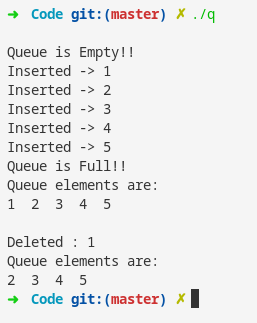
\includegraphics[width=4in]{Images/q.png}
  \label{output:11}
  \caption{Output: 11}
\end{figure}


\pagebreak
\subsection{Temperature Conversion}
\subsubsection{Statement}
Write a program to print the corresponding celsius to Fahrenheit table. Modify the
temperature conversion program to print the table in reverse order, that is from 300 to 0
\subsubsection{Code}
\begin{minted}{c} 
#include <stdio.h>
double to_celcius(int fahr)
{
  return (fahr - 32) * (5.0 / 9.0);
}

int main()
{
  int fahr;
  printf("Fahrenheit     \t Celcius\n");
  for (fahr = 300; fahr >= 0; fahr = fahr - 20)
    printf("%3d \t\t %6.1f\n", fahr, to_celcius(fahr));
}
\end{minted}
\subsubsection{Output}
\begin{figure}[!htb]
  \centering
  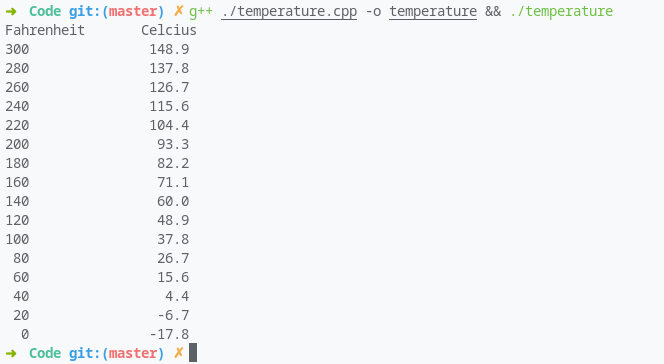
\includegraphics[width=6in]{Images/temperature.png}
  \label{output:12}
  \caption{Output: 12}
\end{figure}


\pagebreak
\subsection{Text in File}
\subsubsection{Statement}
Write a program to count blanks, tabs and newlines
\subsubsection{Code}
\begin{minted}{c} 
#include <stdio.h>

int main()
{
  int blank_char = 0, tab_char = 0, new_line = 0, c;
  printf("Number of blanks, tabs, and newlines:\n");
  printf("Input few words/tab/newlines\n");
  while ((c = getchar()) != EOF)
  {
    switch (c)
    {
    case ' ':
      ++blank_char;
      break;
    case '\t':
      ++tab_char;
      break;
    case '\n':
      ++new_line;
      break;
    default:
      break;
    }
  }
  printf("\nblank=%d, tab=%d, newline=%d\n", blank_char, tab_char, new_line);
}
\end{minted}
\subsubsection{Output}
\begin{figure}[!htb]
  \centering
  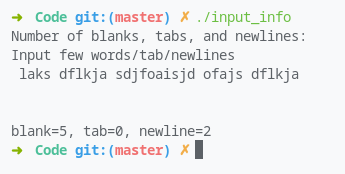
\includegraphics[width=4in]{Images/input_info.png}
  \label{output:13}
  \caption{Output: 13}
\end{figure}


\pagebreak
\subsection{Frequencies}
\subsubsection{Statement}
Write a program to print the histogram of the frequencies of different characters of its input.
\subsubsection{Code}
\begin{minted}{c} 
#include <stdio.h>
#include <string.h>
void histogram(const int offset, const int range)
{
  FILE *file = fopen("./text.txt", "r+");
  int histogram[range];
  memset(histogram, 0, sizeof(histogram)); // initialize 95 spaces for ASCII characters 32 - 127

  int special = 0;

  int c;
  while ((c = fgetc(file)) != EOF)
  {
    if (c < offset || c >= (offset + range))
      special++;
    else
      ++histogram[c - offset];
  }

  for (int i = 0; i < range; ++i)
  {
    c = i + offset;
    printf("%c ", c);
    for (int j = 0; j < histogram[i]; ++j)
      putchar('x');
    putchar('\n');
  }

  printf("- ");
  for (int j = 0; j < special; j++)
    putchar('x');
  putchar('\n');
}

int main(void)
{
  histogram(' ', 95); // ' ' is 32 in ascii
}
\end{minted}
\pagebreak
\subsubsection{Output}
Input Text
\begin{figure}[!htb]
  \centering
  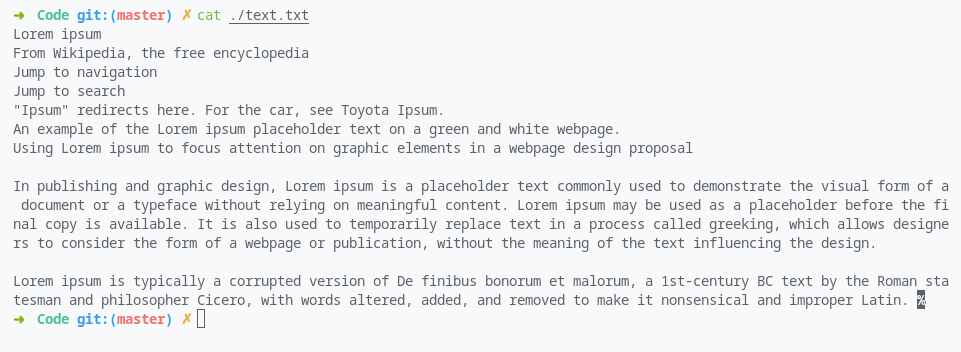
\includegraphics[width=6in]{Images/text.png}
  \label{output:14-Text}
  \caption{Output: 14 - Text}
\end{figure}

Histogram
\begin{figure}[!htb]
  \centering
  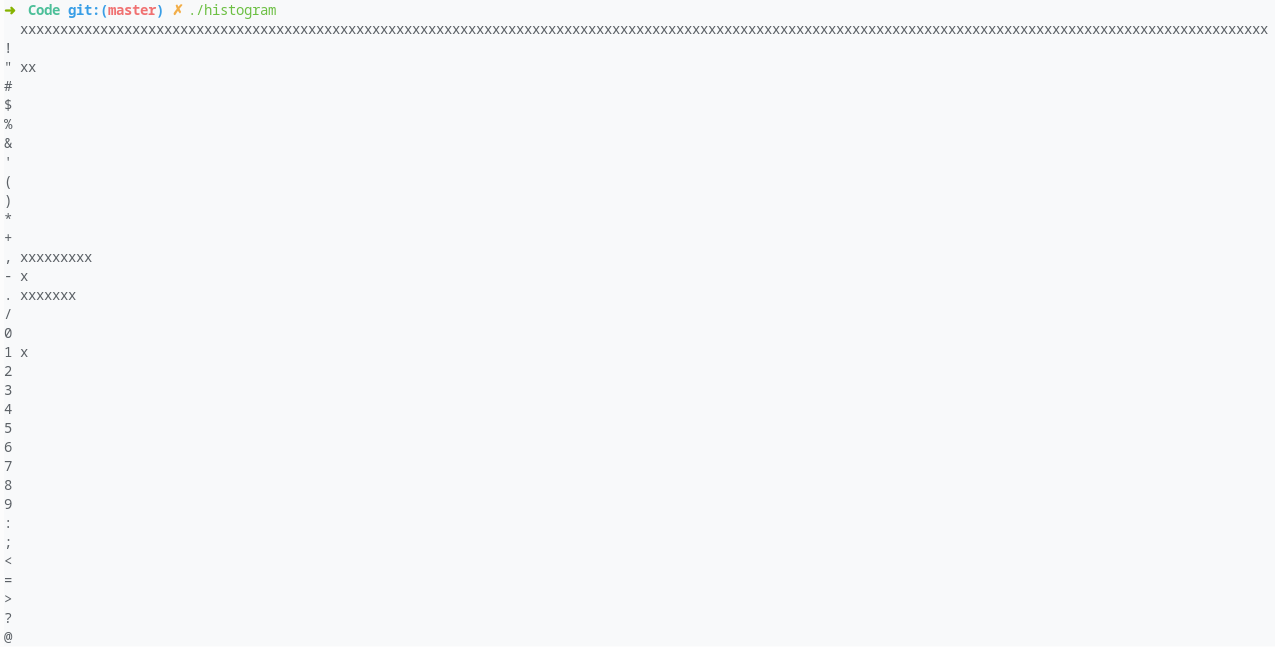
\includegraphics[width=6in]{Images/histogram1.png}
  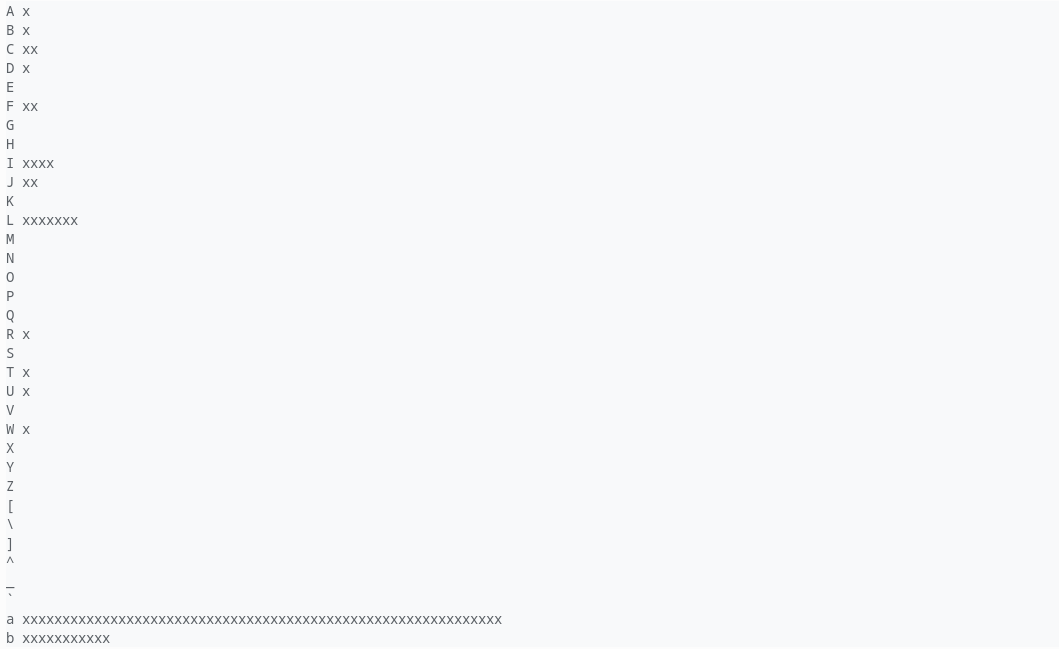
\includegraphics[width=6in]{Images/histogram2.png}
  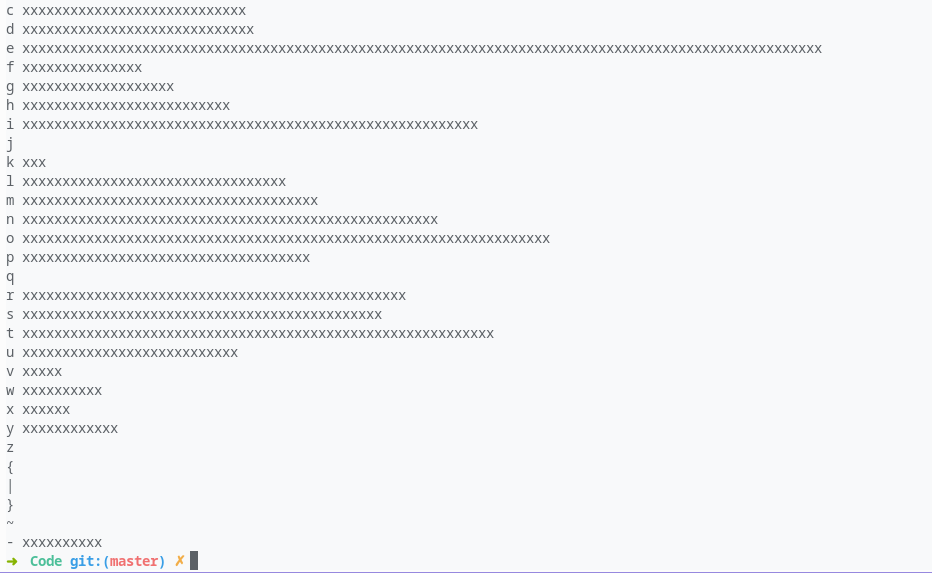
\includegraphics[width=6in]{Images/histogram3.png}
  \label{output:14-Histogram}
  \caption{Output: 14 - Histogram}
\end{figure}